\section{Reversibiliteit en de Derde Hoofdwet}

\begin{definition}[Reversibel proces]
    Een proces is \textbf{reversibel} als het systeem en zijn omgeving na het proces weer in hun oorspronkelijke toestand kunnen worden teruggebracht zonder dat er veranderingen in de omgeving optreden.
\end{definition}
\begin{definition}[Irreversibel proces]
    Een proces is \textbf{irreversibel} als het systeem en zijn omgeving na het proces niet in hun oorspronkelijke toestand kunnen worden teruggebracht zonder dat er veranderingen in de omgeving optreden.
\end{definition}

\subsection{Uitwendige mechanische irreversibiliteit}
\begin{definition}[Dissipatieve effecten]
    \textbf{Dissipatieve effecten} zijn processen waarbij energie wordt omgezet in een vorm die niet meer bruikbaar is voor het verrichten van arbeid, zoals warmte.
    Voorbeelden hiervan zijn wrijving, viscositeit en elektrische weerstand. Men zegt dat er arbeid gedissipeerd wordt.
\end{definition}

\begin{definition}[Perpetuum mobile van de derde soort]   
    Een \textbf{perpetuum mobile van de derde soort} is een hypothetisch apparaat dat in staat is om arbeid te verrichten zonder enige energiebron, door gebruik te maken van dissipatieve effecten. 
    Doordat dit niet in strijd is met de eerste twee wetten van de thermodynamica is er een derde wet nodig.
\end{definition}

\begin{definition}[Externe thermische irreversibiliteit]
    \textbf{Externe thermische irreversibiliteit} is een proces waarbij warmte wordt overgedragen van een warmer object naar een kouder object, zonder dat er enige arbeid wordt verricht. 
    Dit proces is onomkeerbaar omdat het niet mogelijk is om de warmte weer terug te laten stromen van het koudere object naar het warmere object zonder dat er arbeid wordt verricht.
\end{definition}

\begin{definition}[Interne thermische irreversibiliteit]
    \textbf{Interne thermische irreversibiliteit} is een proces waarbij warmte wordt gegenereerd binnen een systeem als gevolg van interne dissipatieve effecten, zoals wrijving of viscositeit. 
    Dit proces is niet omkeerbaar omdat het niet mogelijk is om de gegenereerde warmte weer te verwijderen zonder dat er arbeid wordt verricht.
\end{definition}

\subsection{Voorwaarden reversibiliteit}

\begin{definition}[Reversibiliteit]
    Een proces is \textbf{reversibel} als het voldoet aan de volgende voorwaarden:
    \begin{itemize}
        \item Er zijn geen dissipatieve effecten aanwezig
        \item Het proces verloopt quasistatisch 
    \end{itemize}
\end{definition}

\subsection{Reversibele Adiabatische Oppervlakken}

\begin{postulate}[Carathéodory's postulaat]
    In de nabijheid van een evenwichtstoestand van een systeem, zijn er toestanden die niet kunnen worden bereikt door een adiabatisch proces.
\end{postulate}

Herinner u een algemeen systeem met veralgemeende kracht \(Y\) en veralgemeende verplaatsing \(X\):
\[\dbar Q = dU -YdX\]
met \(U(T_e,X)\) een functie van de empirische temperatuur \(T_e\) en de veralgemeende verplaatsing \(X\).
\[
d U = \left(\frac{\partial U}{\partial T_e}\right)_X dT_e + \left(\frac{\partial U}{\partial X}_{T_e}\right) dX 
\]
\[
dU = \dbar Q + YdX \implies \dbar Q = \left(\frac{\partial U}{\partial T_e}_{X}\right) dT_e + \left[\left(\frac{\partial U}{\partial X}_{T_e}\right)  - Y\right]dX   
\]

Als we nu kijken naar een adiabatisch proces, dan is \(\dbar Q = 0\) en dus:
\[\left(\frac{\partial U}{\partial T_e}_{X}\right) dT_e + \left[\left(\frac{\partial U}{\partial X}_{T_e}\right)  - Y\right]dX = 0\]
Een oplossing voor \(\frac{dT_e}{dX}\) is:
\[\frac{dT_e}{dX} = \frac{Y - \left(\frac{\partial U}{\partial X}_{T_e}\right)}{\left(\frac{\partial U}{\partial T_e}_{X}\right)}\]
Deze oplossing is een adiabatisch oppervlak, de oplossing door een willekeurig punt kan geschreven worden als:
\[
\sigma (T_e ,X) = cst
\]

Een veralgemeend systeem met vijf coördinaten \((T_e, X, X', Y, Y')\) wordt beschreven door:
\[
\dbar Q = dU - YdX - Y'dX'
\]
met als oplossing \(\sigma (T_e, X, X')\), waarvan we de \(\sigma\) later nog zullen definieren als de entropie.

\begin{definition}
    Een \textbf{reversibel adiabatisch oppervlak} is een oppervlak in de toestandruimte van een systeem waarop alle processen adiabatisch en reversibel zijn. 
    Op dit oppervlak kunnen geen dissipatieve effecten optreden, en het proces verloopt quasistatisch. (de ruimte is ook steeds een dimensie lager dan de volledige toestandruimte.)
\end{definition}

RA-oppervlakken kunnen elkaar nooit snijden, want als ze elkaar zouden snijden,
dan zou er een punt zijn waar twee verschillende adiabatische processen elkaar kruisen, wat in strijd is met de definitie van een adiabatisch proces.

\subsection{Integreerbaarheid van dQ}


Herinner u het algemene systeem met vijf coördinaten \((T_e, X, X', Y, Y')\)? We kunnen deze uitschrijven als totale differentiaal van \(U(\sigma, X, X')\):
\[dU = \left(\frac{\partial U}{\partial \sigma}\right)_{X, X'} d\sigma + \left(\frac{\partial U}{\partial X}\right)_{\sigma, X'} dX + \left(\frac{\partial U}{\partial X'}\right)_{\sigma, X} dX'\]
We kunnen dit vergelijken met de algemene uitdrukking van \(\dbar Q\):
\[\dbar Q = dU - YdX - Y'dX' = \left(\frac{\partial U}{\partial \sigma}\right)_{X, X'} d\sigma + \left[\left(\frac{\partial U}{\partial X}\right)_{\sigma, X'} - Y\right] dX + \left[\left(\frac{\partial U}{\partial X'}\right)_{\sigma, X} - Y'\right] dX'\]

Doordat de drie coordinaten \(T_e, X, X'\) onafhankelijk zijn, moeten de volgende voorwaarden gelden:
\[\left(\frac{\partial U}{\partial \sigma}\right)_{X, X'} \neq 0\]
\[\left(\frac{\partial U}{\partial X}\right)_{\sigma, X'} = Y\]
\[\left(\frac{\partial U}{\partial X'}\right)_{\sigma, X} = Y'\]

Zodat kunnen we \(\dbar Q\) schrijven als:
\[\dbar Q = \left(\frac{\partial U}{\partial \sigma}\right)_{X, X'} d\sigma\]
We definieren nu de functie \(\lambda(\sigma)\) als:
\[\lambda(\sigma) = \left(\frac{\partial U}{\partial \sigma}\right)_{X, X'}\]
Zodat we \(\dbar Q\) kunnen schrijven als:
\[\dbar Q = \lambda(\sigma) d\sigma\]

\begin{definition}
    De functie \(\lambda(\sigma)\) wordt de \textbf{integrerende factor} genoemd, omdat het ervoor zorgt dat \(\dbar Q\) een totaal differentiaal wordt. 
    De functie \(\sigma\) wordt de \textbf{entropie} genoemd, en is een functie van de toestand van het systeem die de mate van wanorde of onomkeerbaarheid van een proces beschrijft.
\end{definition}


\begin{derivation}
We beschouwen nu twee systemen met elk drie onafhankelijke coördinaten \((T_e, Y, X)\) en \((T_e', X_H, X_H')\). Ze zijn verondersteld op elk moment in evenwicht te zijn \(T_e = T_e'\).
Samen vormen ze een samengesteld systeem met vijf onafhankelijke coördinaten \((T_e, X_H, X_R, X_H', X_R')\) \footnote{Zoals we net hebben gezien}. 

Het eerste systeem is het hoofdsysteem met coördinaten \((T_e, X_H, X_H')\) en het tweede systeem is het referentiesysteem met coördinaten \((T_e, X_R, X_R')\).
Ze hebben beiden een oplossing van de vorm \(\sigma_H (T_e, X_H, X_H')\) en \(\sigma_R (T_e, X_R, X_R')\) respectievelijk.
We veronderstellen ook dat als de twee systemen een hoeveelheid warmte \(\dbar Q\) uitwisselen, dat \(d\sigma_H\) en \(d\sigma_R\) veranderen met:
\[\dbar Q_H = \lambda_H(\sigma_H) d\sigma_H\] en \[\dbar Q_R = \lambda_R(\sigma_R) d\sigma_R\]
Waar \(\lambda_H\) en \(\lambda_R\) de integrerende factoren zijn van de respectievelijke systemen

In het samengesteld systeem zijn de RA-oppervlakken gegeven door \(\sigma (T_e, X_H, X_H', X_R, X_R') \).

We kunnen de twee systemen  \(X_H'\) en \(X_R'\) uitdrukken in termen van \(T_e,X_H, \sigma_H\) en \(T_e, X_R, \sigma_R\) respectievelijk.
Zodat de coördinaten \(X_H'\) en \(X_R'\) kunnen worden geëlimineerd uit de vergelijking van het samengestelde systeem, en we kunnen schrijven:
\[\sigma_c = \sigma_c (T_e, X_H, X_R, \sigma_H, \sigma_R) \]
Waar \(\lambda_c\) een functie is die de relatie tussen de entropieën van de twee systemen beschrijft. 
En analoog als daarnet \( \dbar Q_c = \lambda_c(\sigma) d\sigma\) kunnen we schrijven:

We kunnen dus schrijven:
\tiny
\[d\sigma_c = \left(\frac{\partial \sigma_c}{\partial \sigma_H}\right)_{T_e, X_H, \sigma_R , X_R} d\sigma_H
 + \left(\frac{\partial \sigma_c}{\partial \sigma_R}\right)_{ T_e, X_H, \sigma_H, X_R} d\sigma_R
+ \left(\frac{\partial \sigma_c}{\partial T_e}\right)_{X_H, \sigma_H, X_R, \sigma_R} dT_e 
+ \left( \frac{\partial \sigma_c}{\partial X_H} \right)_{T_e, \sigma_H, \sigma_R, X_R} dX_H
+ \left(\frac{\partial \sigma_c}{\partial X_R} \right)_{T_e, \sigma_H, \sigma_R, X_H} dX_R\]
\normalsize

Veronderstel dat een reversibel proces de warmteoverdracht \(\dbar Q_c\) tussen het warmtereservoir en het gecombineerde systeem opsplitst in een warmteoverdracht \(\dbar Q\)
naar het hoofdsysteem en een warmteoverdracht \(\dbar Q_R\) naar het referentiesysteem, zodat:
\begin{align*}
    \dbar Q_c &= \dbar Q + \dbar Q_R\\
    \implies \lambda_c d\sigma_c &= \lambda_H d\sigma_H + \lambda_R d\sigma_R\\
    \implies d\sigma_c &= \frac{\lambda_H d\sigma_H}{\lambda_c} + \frac{\lambda_R d\sigma_R}{\lambda_c}
\end{align*}
Pluggen we dit in onze hele lange vergelijking van nu net, dan vinden we:
\begin{align*}
    \frac{\lambda_H}{\lambda_c} &= \left(\frac{\partial \sigma_c}{\partial \sigma_H}\right)_{T_e, X_H, \sigma_R , X_R}
    \implies \frac{\lambda_H}{\lambda_c} = \frac{\partial \sigma_c}{\partial \sigma_H} \\
    \frac{\lambda_R}{\lambda_c} &= \left(\frac{\partial \sigma_c}{\partial \sigma_R}\right)_{ T_e, X_H, \sigma_H, X_R}
    \implies \frac{\lambda_R}{\lambda_c} = \frac{\partial \sigma_c}{\partial \sigma_R} \\
    0 &= \left(\frac{\partial \sigma_c}{\partial T_e}\right)_{X_H, \sigma_H, X_R, \sigma_R} 
    \implies \frac{\partial \sigma_c}{\partial T_e} = 0 \\
    0 &= \left( \frac{\partial \sigma_c}{\partial X_H} \right)_{T_e, \sigma_H, \sigma_R, X_R} 
    \implies \frac{\partial \sigma_c}{\partial X_H} = 0 \\
    0 &= \left(\frac{\partial \sigma_c}{\partial X_R} \right)_{T_e, \sigma_H, \sigma_R, X_H}
    \implies \frac{\partial \sigma_c}{\partial X_R} = 0
\end{align*}

Dit zegt ons iets heel belangrijks, namelijk \(\sigma_c\) van de twee systemen gerelateerd zijn door een functie van de entropieën van de twee systemen, en dat \textbf{deze functie alleen afhankelijk is van de entropieën (nu nog \(\sigma_H\) en \(\sigma_R\)) en niet van de andere coördinaten (zoals \(T_e\), \(X_H\), en \(X_R\) zoals net aangetoond).}

Dus we kunnen \(\sigma_c\) schrijven als:
\[\sigma_c = \sigma_c(\sigma_H, \sigma_R)\]
met zoals net berekend:
\[\frac{\lambda_H}{\lambda_c} = \frac{\partial \sigma_c}{\partial \sigma_H}\] en \[\frac{\lambda_R}{\lambda_c} = \frac{\partial \sigma_c}{\partial \sigma_R}\]
Dus de deze verhoudingen zijn niet afhankelijk van de andere coördinaten, maar alleen van de entropieën van de twee systemen.

Maar waarvan zijn ze nu wel nog afhankelijk?
\begin{align*}
    \lambda_H &= \phi(T_e, X_H, X_R) f(\sigma_H) = \phi(T_e)f(\sigma_H) \\
    \lambda_R &= \phi(T_e, X_H, X_R) g(\sigma_R) = \phi(T_e)g(\sigma_R) \\
    \sigma_c &= \sigma_c(T_e, X_H, X_R) h(\sigma_H, \sigma_R) = \phi(T_e)h(\sigma_H, \sigma_R) \\ 
\end{align*}
Doordat \(\lambda_H\) niet afhankelijk is van \(X_R\) en \(\lambda_R\) niet van \(X_H\), moet \(\phi(T_e)\) enkel afhankelijk zijn van \(T_e\).
Het is noodzakelijk dat \(\phi(T_e)\) afhankelijk is van \(T_e\), want als dat niet het geval zou zijn, dan zou \(\phi = 1\) gesteld kunnen worden, en dan zou in \(\dbar Q = \lambda(\sigma) d\sigma = f(\sigma)d\sigma\) het lid \(\dbar Q\) geen totale differentiaal zijn en het andere lid dat wet is.

Nu kunnen we zeggen dat voor een systeem met willekeurig aantal coördinaten:
\[\dbar Q = \phi(T_e)f(\sigma) d\sigma\]
met \(f(\sigma)d\sigma\) een totale differentiaal, en \(\frac{1}{\phi(T_e)}\) de integrerende factor.
\qed
\end{derivation}

\begin{postulate}
    Er bestaat steeds een integrerende factor \(\frac{1}{\phi(T_e)}\) zodat \(\dbar Q\) een totaal differentiaal wordt, en deze integrerende factor is alleen afhankelijk van de empirische temperatuur \(T_e\).
\end{postulate}

\subsection{De Kelvintemperatuurschaal en de Derde Hoofdwet}

Veronderstel dat een reversibele isotherme hoeveelheid warmte \(\dbar Q\) wordt uitgewisseld tussen ons systeem en een warmtereservoir op \(T_e\). 
Ons systeem gaat van toestand b (op RA-oppervlak \(\sigma_1\)) naar toestand c (op RA-oppervlak \(\sigma_2\)):
\[
Q = \phi(T_e) \int_{\sigma_1}^{\sigma_2}f(\sigma)d\sigma  \qquad (T_e = cst)
\]

Voor de figuur verwijs ik jullie naar de cursus, aangezien ik deze niet kan overnemen vanwege auteursrechten. 
Het is de Carnot cyclus volgens 2 reversibele isotherme processen en 2 reversibele adiabatische processen in een 3D plot met veralgemeende coordinaten \(T_e, X, X'\).

Het reversibele endotherme proces van toestand \(a \to d \) bij \(T_e'\) wordt de warmteoverdracht \(Q'\):
\[
Q' = \phi(T_e') \int_{\sigma_1}^{\sigma_2}f(\sigma)d\sigma  \qquad (T_e' = cst)
\]
De verhouding geeft ons:
\[\frac{Q}{Q'} = \frac{\phi(T_e)}{\phi(T_e')}\]

We definieren nu de \textbf{Kelvintemperatuurschaal} als:
\begin{equation}
    \label{eq:Kelvintemp}
    \frac{Q}{Q'} = \frac{T_k}{T_k'}
\end{equation}
waarbij de \(_k\) voor Kelvin staat.

Twee temperaturen op de Kelvinschaal verhouden zich zoals de warmteoverdracht tussen twee RA-oppervlakken bij die temperaturen.
\textbf{De temperatuur op de Kelvinschaal is onafhankelijk van de stof (met zijn thermometrische eigenschappen).} 
\(Q\) speelt de rol van thermometrische eigenschap, maar hangt niet af van de specifieke stof, maar alleen van de temperatuur.

\(T=0\) op de Kelvinschaal is het absolute nulpunt, en dit is een onbereikbare temperatuur.
\begin{postulate}
    Als een stelsel een reversibel isotherm proces ondergaat, waarbij geen warmte wordt uitgewisseld, dan is de temperatuur van het stelsel gelijk aan het absolute nulpunt \(T=0\).
\end{postulate}

\begin{postulate}[Derde hoofdwet van de thermodynamica (Nernst)]
    Er is geen enkel proces mogelijk, dat met een eindig aantal stappen, toelaat het absolute nulpunt \(T=0\) te bereiken.
\end{postulate}

De \textbf{Carnotcyclus} bestaat uit twee isotherme processen en twee adiabatische processen, en is een voorbeeld van een reversibele cyclus (dus puur theoretisch).

\subsection{Gelijkheid Ideaal-gastemperatuur en de Kelvintemperatuur}
\begin{figure}[h]
    \centering
    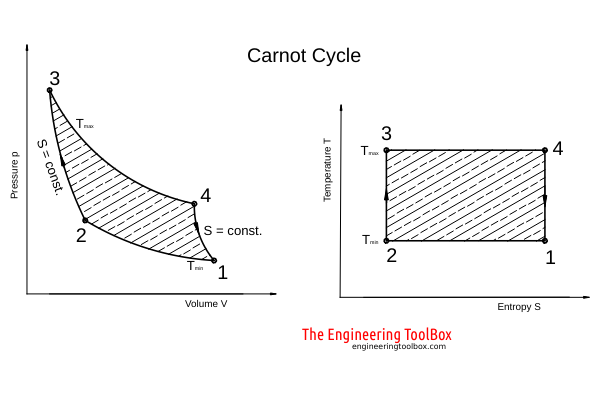
\includegraphics[width=0.5\textwidth]{Foto's-Figuren/carnot_cycle.png}
    \caption{\tiny \copyright{(The Engineering ToolBox, 2008). Carnot Cycle Efficiency. [online] Available at: \url{https://www.engineeringtoolbox.com/carnot-efficiency-d_1047.html} [Accessed 14 May 2026].}}
    \label{Fig:carnot-cycl}
\end{figure}
\begin{derivation}
    Voor een ideaal gas geldt:
    \[\dbar Q = C_V dT + PdV\]
    We passen dit toe op de isotherm \( 1 \to 2 \):
    \[
    Q = \int_{V_1}^{V_2} P dV = nRT \ln\left(\frac{V_2}{V_1}\right) \qquad (T = cst)
    \]
    En op de isotherm \( 3 \to 4 \):
    \[Q' = \int_{V_3}^{V_4} P dV = nRT' \ln\left(\frac{V_4}{V_3}\right) \qquad (T' = cst)\]
    De verhouding geeft ons:
    \[\frac{Q}{Q'} = \frac{T}{T'} \frac{\ln\left(\frac{V_2}{V_1}\right)}{\ln\left(\frac{V_4}{V_3}\right)}\]
    Maar omdat \(2 \to 3\) en \(1 \to 4\) adiabatische processen zijn, geldt:
    \[C_VdT = -PdV = -\frac{nRT}{V}dV\]
    \[\implies \frac{1}{nR}\int_{T'}^{T} \frac{dT}{T} = \ln \frac{V_2}{V_3}\]
    en
    \[\frac{1}{nR}\int_{T}^{T'} \frac{dT}{T} = \ln \frac{V_1}{V_4}\]
    Hieruit volgt dat:
    \[\ln\frac{V_2}{V_3} = \ln\frac{V_1}{V_4} \implies \frac{V_2}{V_3} = \frac{V_1}{V_4} 
    \implies \frac{V_2}{V_1} = \frac{V_4}{V_3 }\]
    Pluggen we dit terug in de verhouding van \(Q\) en \(Q'\) van de kelvin temperatuur in \eqref{eq:Kelvintemp}, dan vinden we:
    \[\frac{Q}{Q'} = \frac{T}{T'}\]
    Wat precies de verhouding is van de Kelvintemperaturen \(T_k\) en \(T_k'\) zoals we net hebben gedefinieerd.
    Als we \(T_k'\) en \(T'\) gelijk stellen aan 273,15 K dan:
    \[T = T_k\]
    De Kelvintemperatuur (onafhankelijk van de stof) is dus gelijk aan de ideale gastemperatuur (afhankelijk van de stof).
    \qed
\end{derivation}
    